%% ========================================================================
%%							NNLS
%% ========================================================================


\chapter{Non-negative least squares (NNLS)}
\label{cha:NNLS}

Another way to find a grouped portfolio that minimizes the deviation defined in formula (\ref{eq:objective_function}) is to solve the problem using mathematical optimization methods. The goal is to find a subset of the portfolio and scale it in way so that the square deviation becomes minimal. Of course, this approach must ensure that scaling is only possible in the positive direction. This means that it makes no sense to have a negative policy in the grouped portfolio, because it cannot be defined, not to mention explained logically. 

\begin{definition}[Non-negative least squares]\label{def:NNLS}
	Let $P \subset \V$ be a portfolio, $A \in \R^{m \times n}$ the matrix with the corresponding cashflows and $b \in \R^m$ the vector with the summed cashflows. Then $x \in \R^n$, the vector of scaling, should be optimized such that:  
	\begin{equation}\label{eq:NNLS}
		\begin{aligned}
			\argmin_x \lVert Ax -b \rVert_2^2 \\
			\text{subject to } x \geq 0
		\end{aligned}
	\end{equation}
\end{definition}

\begin{remark}
	\leavevmode % needed for items to start in new line after remark.
	\makeatletter
	\@nobreaktrue
	\makeatother
	\begin{itemize}
		\item 	The entries of the vector $x$ are the so-called scaling values for the cashflows in matrix $A$. Each entry $x_i, i \in \{1,...n\}$ that is greater than zero scales to the $i$-th column of matrix $A$ where column $i$ represents the cashflows of the $i$-th policy of the portfolio.
		\item 	It should be noted that this approach optimizes cashflows, not policies. Since there is a one-to-one relationship between cashflows and policies, the scaling factors cannot only be used to scale the cashflows but also to scale the policies in order to create a grouped portfolio. 
		\item 	Scaling policies can also involve risks, as a policy that is scaled by a factor of 2 will not necessarily produce cash flows that are also increased by a factor of 2. This can be attributed to the fact that, for example, non-linearities occur due to discount effects for higher premiums in the tariff.
	\end{itemize}
\end{remark}

\begin{remark}
	The number of policies in the grouped portfolio corresponds exactly to the number of entires greater than zero in the vector $x$.
\end{remark}

One of the well known algorithms for solving the non-negative least square problem is that of Lawson and Hanson, which uses an active set method. The steps necessary for solving that problem are given in \cite{lawson}. Additionally to those parameters defined in definition \ref{def:NNLS} one also needs a real value variable $\epsilon$ as a stopping criterion.

\begin{algorithm}
	\caption{Non-negative least squares \cite{lawson}}\label{alg:NNLS}
	\begin{algorithmic}
		\\
		\begin{enumerate}
			\item Set $P = \emptyset$, $R = \{1, ..., n\}$, $x$ = $0_{n \times 1}$
			\item Compute $w = A^\top(b - Ax)$.
			\item While $R \neq \emptyset$ and $max(w) > \epsilon$
			\begin{enumerate}[label=\emph{\alph*})]
				\item Find index $j \in R$ such that $w_j = max\{w_t, t \in R\}$.
				\item Move the index $j$ from $R$ to $P$.
				\item Let $A^P$ be $A$ restricted to the variables included in $P$.
				\item Let $s$ be a vector of same length as $x$. Let $s^P$ denote the sub-vector with indexes from $P$, and let $s^R$ denote the sub-vector with indexes from $R$.
				\item Compute $s^P = ((A^P)^\top A^P)^{-1} (A^P)^\top b$
				\item Set $s^R = 0$.
				\item While $min(s^P) \leq 0$
				\begin{enumerate}
					\item Set $\alpha_k = min\frac{x_i}{x_i - s_i}$ for $i$ in $P$ where $s_i \leq 0$
					\item Set $x = x + \alpha_k(s-x)$
					\item Move from $P$ to $R$ all indices $k \in P$ for which $x_k = 0$.
					\item Compute $s^P = ((A^P)^\top A^P)^{-1} (A^P)^\top b$
					\item Set $s^R = 0$
				\end{enumerate}
				\item Set $x$ to $s$
				\item Compute $w = A^\top(b - Ax)$.
			\end{enumerate}
		\end{enumerate}
	\end{algorithmic}
\end{algorithm}

Algorithm \ref{alg:NNLS} consists, apart from the initialization, of a main loop and an inner loop. The loops are highlighted by indentations and start at step 3 and step g) respectively. If for a variable reference is made to those indices of the variable which are contained in the set $R$, then these entries are 0. All indexes that exist in the set P, by contrast, have nonzero values. If such a variable has a negative value, the algorithm either moves it to the positive value range or sets it to zero. By setting a variable to zero, the index is also shifted from the set $P$ to the set $R$. This ensures that the following condition is met at the end of the algorithm.   
\begin{align}\label{equ:final_conditions}
\begin{split}
	x_j &> 0, \quad j \in P \\
	x_j &= 0, \quad j \in R
\end{split}
\end{align}



\begin{remark}\label{rem:gradient}
	Let $f(x) = \lVert Ax -b \rVert_2^2$ be the function, then the gradient is given by: 
	\begin{equation*}
		\nabla f(x) = \nabla \lVert Ax -b \rVert_2^2 = A^\top(Ax-b)
	\end{equation*}
	
	\begin{align*}
		\nabla \lVert Ax -b \rVert_2^2	&= \nabla (Ax-b)^\top (Ax-b) \\
										&= \nabla (x^\top A^\top - b^\top)(Ax-b) \\
										&= \nabla (x^\top A^\top Ax - x^\top A^\top b - b^\top Ax + b^\top b) \\
										&= \nabla (x^\top A^\top Ax - 2x^\top A^\top b + b^\top b) \\
										&= 2 (A^\top A x - A^\top b) \\
										&= 2A^\top (Ax - b)
	\end{align*}
\end{remark}

As shown in remark \ref{rem:gradient}, step 2 of algorithm \ref{alg:NNLS} calculates the negative gradient of the ordinary least squares problem. In the next step it is checked whether the inner loop still has to be executed or not. If the index set $R$ correspond to the empty set then all indexes are already in $P$ which means that all entries of $x$ are positive (see formula (\ref{equ:final_conditions})). This case is not desirable, as no compression can be achieved. If $max(w) \leq \epsilon$ is satisfied, the gradient has no entry large enough, so that an substantial improvement can be achieved and the algorithm has reached the optimum. If one of the two conditions in step 3) is fulfilled, the main loop is executed. 

The main loop starts with searching for the index of the gradient that is not yet present in the set $P$ and has the highest value. After this index has been moved from the set $R$ to the set $P$, the solution of a restricted least square problem is calculated in step e). This least squares problem is limited to the columns of the matrix $A$ whose indices occur in the set $P$. The result is then a vector of dimension $P$ which is indicated by the notation $s^P$. To get a solution vector of the dimension $n$, the $n - \vert P \vert = \vert R \vert$ entries $s^R$ of the vector $s$ are filled with 0 - see step f). 

\begin{example}
	Based on algorithm \ref{alg:NNLS}, be $n = 15$, $P = \{2, 3, 4, 5, 7, 9\}$ and  $R = P^c = \{1, 6, 8, 10, 11, 12, 13, 14, 15\}$ then
	\begin{equation*}
		\begin{aligned}[c]	
		s = 
		\left( 
		\begin{array}{c}
		s_{1} \\
		s_{2} \\
		\vdots\\
		s_{15}\\
		\end{array}
		\right)	
		\end{aligned}
		\qquad
		\begin{aligned}[c]
		s^P = 
		\left( 
		\begin{array}{c}
		s_{2} \\
		s_{3} \\
		s_{4} \\
		s_{5} \\
		s_{7} \\
		s_{9} \\
		\end{array}
		\right)	
		\end{aligned}
		\qquad
		\begin{aligned}[c]
		s^R = 
		\left( 
		\begin{array}{c}
		s_{1} \\
		s_{6} \\
		s_{8} \\
		s_{10} \\
		\vdots \\
		s_{15} \\
		\end{array}
		\right)	
		\end{aligned}	
	\end{equation*}
\end{example}

If all components of this least square solution (i.e. $s^P$) are positive a new solution has been found and the solution vector $x$ is overwritten with $s$ as seen in step h). In step i) a recalculation of the gradient with the solution $x$, adapted in the previous step, is carried out and the main loop is restarted by checking the conditions in step 3. 

If there are non positive entries in the solution of the restricted least squares problem computed in step e), the inner loop is executed. Basically, negative entries in the result vector $s^P$ would lead to a new solution vector $x$ which would also have negative entries without further adjustments, resulting in an undesired solution since $x$ must be non-negative (i.e $x \geq 0$). Therefore, based on the current solution vector $x$ which has only positive entries, a shift is carried out by using $s^P$. In the first step the index $k \in P$ is determined which leads to the smallest scaling factor $\alpha_k$. The current solution vector $x$ is then shifted by using this factor which causes the entry $x_k$ to be zero after the shift. The index $k$ can thus be moved from set $P$ back to set $R$ because the corresponding entry $x_k$ is zero after the shift. In the unlikely event that several entries of the new solution vector $x$ were changed to zero as a result of the shift, all these indexes must of course be moved from set $P$ to set $R$ (see iii.). Based on the new set $P$, a new limited least squares problem will be solved and the inner loop will be redone if necessary.

\begin{remark}
	Since $x_i \geq 0$ at all times and $s_j \leq 0$ within the inner loop, the scaling factor is bounded by $0 \leq \alpha_k \leq 1$.  
\end{remark}

\begin{remark}
	Within the inner loop, at least one index $k$ per iteration is transferred from the set $P$ to the set $R$.  As a result, with each pass of the inner loop, the number of entries in the solution vector $x$ that are not equal to zero is reduced by at least one. Since the cardinality of the set P is finite, it is also determined how often the inner loop is run through at the most, namely $|P| - 1$ times.
\end{remark}

As stated in \cite[p.~163]{lawson}, for many examples the steps of the outer loop are simply repeated by adding another positive coefficient to the solution vector $x$ until one of the termination criteria in step 3 are fulfilled. This observation may be correct for many different application areas, but must be verified with respect to the policy data being optimized. For this purpose, a standard portfolio of policies is used in which the development of the vector $x$ is analyzed. The test portfolio consists of 20.000 randomly selected policies using 351 cash flows for each policy. 

Figure (\ref{fig:iterations}) shows how the number of non-negative entries of the solution vector $x$ evolves. After the algorithm is started with an initialization, the solution vector $x$ only has entries that are zero and the next step is to execute the main loop for the first time. So the graph starts in (0,0). After passing through the main loop for the first time, the first entry of $x$ became a positive value and the graph displays this as the point (1,1). Also the next 9 passes of the main loop run exactly as just described so that after 10 iterations 10 entries of $x$ are not equal to zero and the graph is at (10,10). In the next pass of the main loop, the solution $s^P$, see step e), of the restricted least squares problem becomes for the first time not positive for at least one entry and the inner loop is executed. When entering the inner loop, $s^P$ has the dimension 11. Within the inner loop, as explained above, a shift is performed and the index $k$ is shifted from the set $P$ to the set $R$. Due to this shift of the index and the subsequent recalculation of the now dimensionally reduced least squares problem (see iv.), $s^P$ now has only dimension 10. Since none of these 10 entries is not positive, the inner loop is now left. The solution vector still has only 10 positive entries after the 11 iteration and therefore the point (11,10) results. The just described phenomenon that the inner loop is left again after one iteration, since all negative entries have been removed, can be observed in figure (\ref{fig:iterations}) more often. This is exactly the case when a horizontal line is present. In the above example, it is also easy to see that this phenomenon of horizontal lines occurs more frequently after about 50 iterations. This can be explained by the fact that at the beginning of an optimization the limited least square problem which need to be solved has a small dimension and therefore it is less likely to get negative solution values. In the progress of the optimization, the achievable improvements of the objective function become smaller and smaller on also the cardinality of the set $P$ increases. The last feature in figure (\ref{fig:iterations}) that can be observed is that of a descending line. This case occurs for the first time at the transition from iteration 28 to iteration 29. In iteration 29 the solution vector of the limited least square problem $s^P$ has entries that are not positive such as in the case described previously. The difference to before is that the inner loop is not left after one iteration. So there are several loop cycles required to adapt all negative entries by shifting. In the particular case of iteration 29, the inner loop is executed exactly twice until all entries of $s^P$ are positive. Since with each pass of the inner loop the number of positive entries of the solution vector $x$ is reduced by one, a descending line results after 2 passes. It is therefore clear that the steepness of the descent is a measure of how often the inner loop has been looped before all entries were positive. 


\begin{figure}
	\centering
	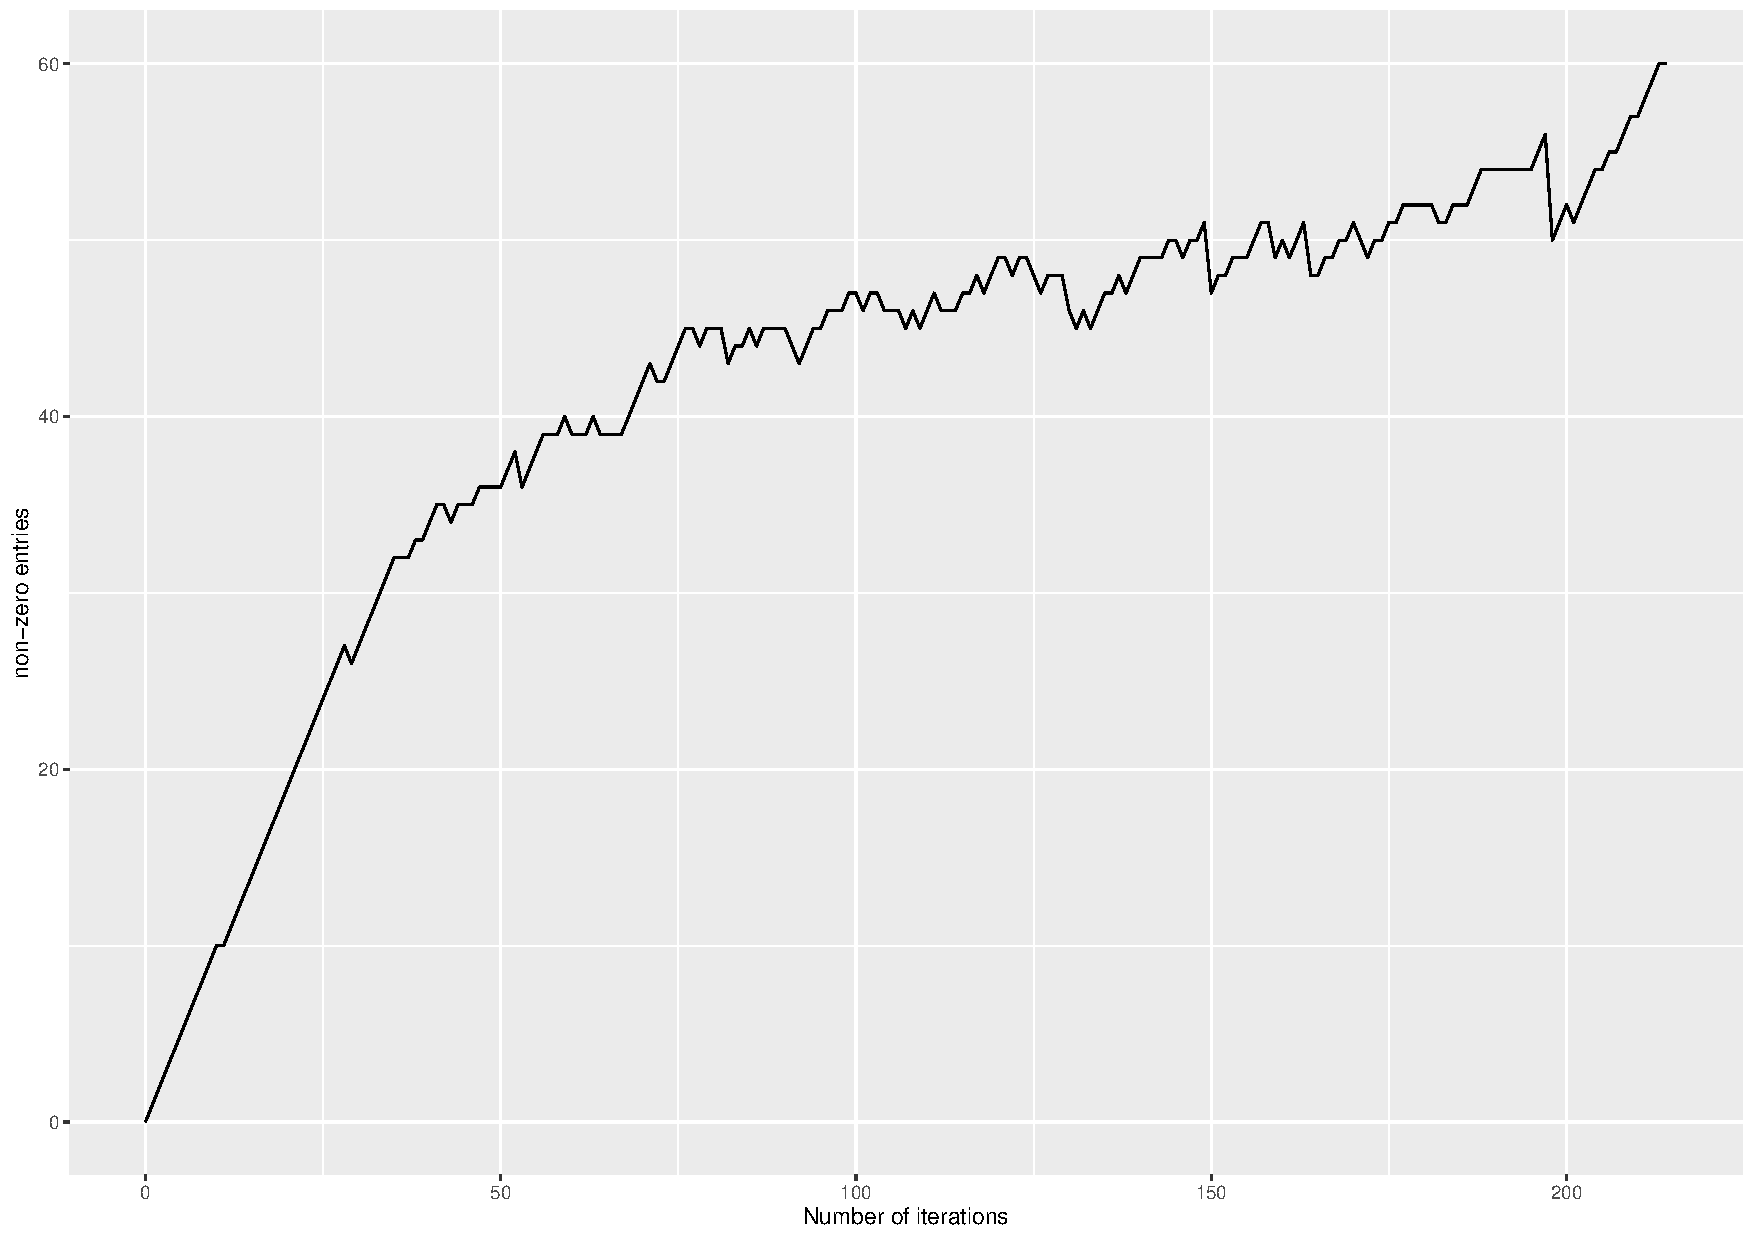
\includegraphics[width=\textwidth]{figures/chapter_NNLS/number_iterations}
	\caption{Development of the non-negative entries of the solution vector $x$ based on the number of iterations.}
	\label{fig:iterations}
\end{figure}

If not the number of non-negative entries is considered but the development of \ref{eq:NNLS} for each iteration, a similar picture emerges. Graph (\ref{fig:residuals}) shows the logarithmic sum of the squared deviations between the fitted cashflows $Ax$ and the reference cashflows $b$. The graph is monotonously falling and can be compared in its characteristics with the previous figure (\ref{fig:iterations}). Starting with the initialization, the solution vector $x$ has only zero entries and therefore $\lVert Ax -b \rVert_2^2$ reduces to $\lVert b \rVert_2^2$ which gives the first data point of the graph at (0, 2.13e+20). Especially at the beginning of the optimization, a new non-negative entry in $x$ is added with each iteration, as seen in figure (\ref{fig:iterations}). This is also reflected in the fact that in figure (\ref{fig:residuals}) the deviation falls significantly for the first iteration. From iteration 50 on there is a clear flattening of the curve which indicates that from then on the improvements of the target function are no longer possible to the same extent as at the beginning of the optimization. This is also confirmed by the fact that after 25\% of the iterations 99.9\% of the reduction of the target function has already taken place. The remaining 0.1\% improvement to the final optimized value of problem (\ref{eq:NNLS}) then take place in the last 75\% of the iterations. Since, as described in more detail in the next section, the inversion of matrices is one of the most time-consuming steps in terms of execution time, it can be useful to cancel an optimization prematurely.  A large part of the computing time could be saved and at the same time only a fraction of the optimization quality would be lost. 

\begin{figure}
	\centering
	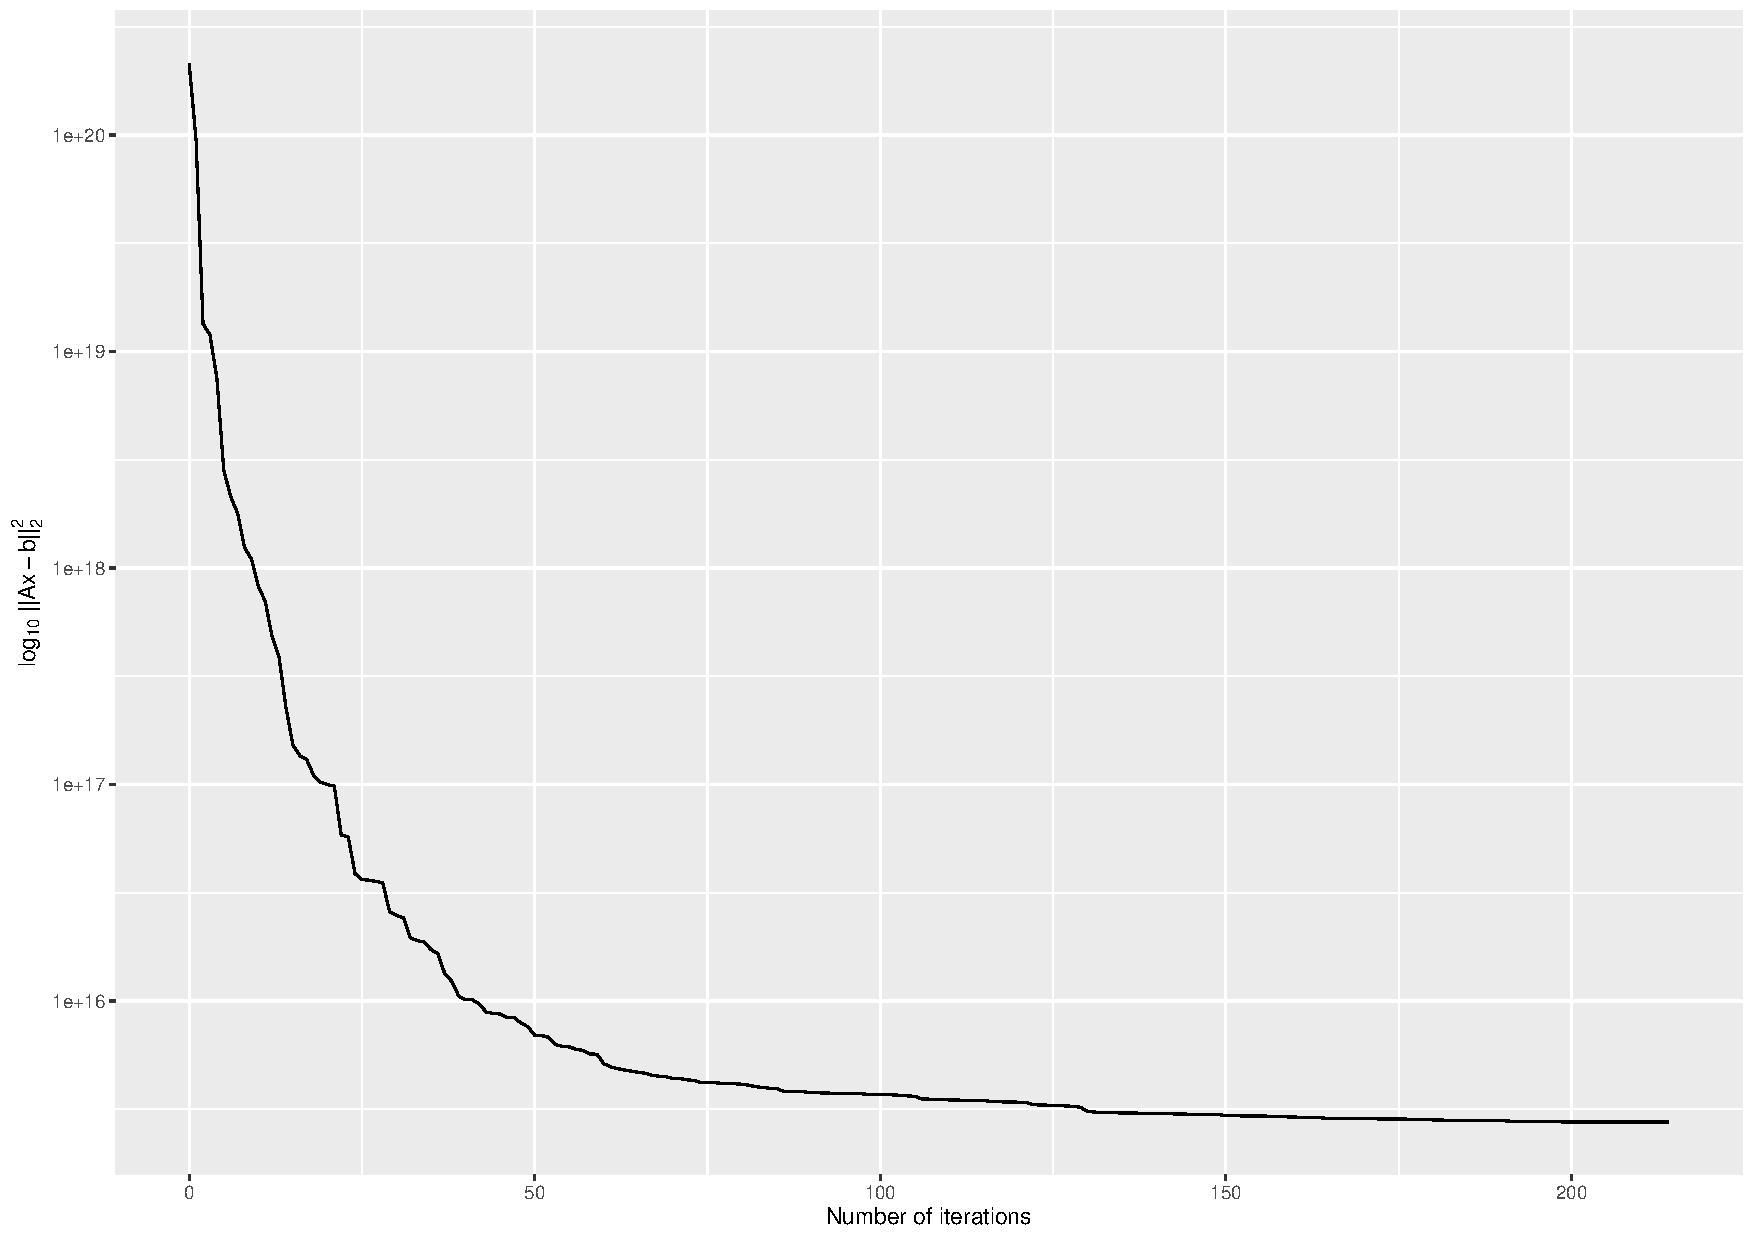
\includegraphics[width=\textwidth]{figures/chapter_NNLS/residuals}
	\caption{Development of the deviance based on the number of iterations.}
	\label{fig:residuals}
\end{figure}

\section{Numerical Aspects}
As evident in figure (\ref{fig:iterations}) as well as figure (\ref{fig:residuals}), the optimization is stopped after 214 iterations. The reason for this is neither that a sufficiently large gradient is no longer available nor that the set $R$ is empty. So all conditions of the main loop stated in step 3 of algorithm \ref{alg:NNLS} are still fulfilled. 
Rather, a stable state has occurred which does not allow any further improvement of the results. Reaching a stable state during an optimization is one of several reasons for an optimization to stop.

Facing a stable state involves a very special case of index shifts between the sets $R$ and $P$, which must be handled separately by the algorithm. Starting from a gradient calculated in step i), the new index $j$ in $R$ is searched for which has the maximum gradient. This new index is then moved from the set $R$ to the set $P$ and the constrained least squares problem is calculated as specified in step e). Since the vector $s^P$ now has exactly one negative entry, the inner loop must be entered in the next step. It turns out that exactly that index $j$ of $s$ is negative which was added by the shift from $j$ to $P$ in the last main loop. 
Since the corresponding entry $x_j$ is zero and $s$ has only one negative entry, the scaling factor $\alpha$ also has a value of zero. This leads to the fact that the shift specified in step ii. has no effect and the solution vector $x$ remains the same. In step iii. the previously determined index $j$ will then be shifted back from the set $P$ to the set $R$. In the next iteration of the main loop, the index with the largest gradient is found again as the previously moved index $j$. This will lead to what has just been described, resulting in an infinite loop. A case such as this therefore only occurs if the following two conditions occur simultaneously: 

\begin{enumerate}
	\item The solution vector $s^P$ of the constrained least squares problem has one negative entry.
	\item This negative entry is in vector $s$ exactly at the index that was transferred from set $R$ to set $P$ in the current loop pass in step b).
\end{enumerate}


\begin{remark}
	If the stopping reason of the optimization algorithm is the reaching of a stable status, the number of non-negative entries of the solution vector $x$ must be equal for the last two iterations. This means that in figure (\ref{fig:iterations}) the graph has to end with a horizontal line.
\end{remark}

Another reason that can lead to an unplanned termination of the optimization algorithm is related to solving process of the restricted least squares problem in step e) and iv). In these steps the solution of the constrained least squares problem is calculated which requires the use of an inverse matrix. If the inverse of $((A^P)^\top A^P)^{-1}$ does not exist, an alternative solution has to be found. The most practicable approach is to test whether an inverse exists using the determinant of $(A^P)^\top A^P$. If this is not the case, remove the just added index $j$ from the set $P$ and replace it with a $j'$ which has the second largest gradient. 
Not only the existence of the inverse matrix is important but also its numerical stability. Therefore it should be ensured that with a small change of the matrix $A$, the inverse matrix $A^{-1}$ do not change significantly in order to get stable results. To determine whether the inversion of a matrix $A$ is numerically stable, a new concept must be introduced which characterizes the numerical stability.



\begin{definition}
	Let $V$ and $W$ be normed vector spaces and $f:V \to W$ a linear operator. Then the operator norm is given by: 
	\begin{align}\label{eq:operator_Norm}
		\lVert f \rVert := \sup_{x \in V \setminus \{0\}} \frac{\lVert f(x) \rVert_W}{\lVert x \rVert_V} = \sup_{\lVert x \rVert_{V} = 1} \lVert f(x) \rVert_V
	\end{align}
\end{definition}

\begin{remark}
	Since every real valued matrix $A \in \R^{m \times n}$ corresponds to a linear map from $\R^n$ to $R^m$, each pair of norms induces an operator norm. In the special case of choosing the Euclidean norm for both vector spaces, (\ref{eq:operator_Norm}) simplifies to:
	\begin{align}\label{eq:matrix_Norm}
		\lVert A \rVert_2 := \max_{x \neq 0} \frac{\lVert Ax \rVert_2}{\lVert x \rVert_2} = \max_{\lVert x \rVert_{2 = 1}} \lVert Ax \rVert_2
	\end{align}	
	which is a naturally induced matrix norm called spectral norm. 
\end{remark}

The natural matrix norm thus vividly corresponds to the greatest possible stretching factor, which results from the application of the linear mapping (i.e. matrix) to a unit vector.

\begin{remark}
	The naturally induced matrix norm satisfies the three norm axioms:
	\begin{itemize}
		\item $\lVert A \rVert = 0$ iff $A = 0$ \hfill (being definite)
		\item $\lVert \alpha A \rVert = |\alpha| \lVert A \rVert$ \hfill (being absolutely homogeneous)
		\item $\lVert A + B  \rVert \leq \lVert A \rVert + \lVert B \rVert$ \hfill (being sub-additive)
	\end{itemize}
\end{remark}

\begin{remark}[\cite{stewart1998matrix}]
	The 2-norm has the following properties:
	\begin{enumerate}
		\item $\lVert A \rVert_2$ = $\sigma_{max}(A)$ \hfill largest singular value of $A$
		\item $\lVert A \rVert_2^2$ = $\lambda_{max}(A^T A)$ \hfill largest eigenvalue value of $A^T A$
		\item $\lVert A \rVert_2 = \lVert A^T \rVert_2$
	\end{enumerate}
\end{remark}

\begin{definition}
	Let $A \in \R^{m \times n}$ be a matrix and $\lVert . \rVert$ a matrix norm. Then the condition number of $A$ is defined as:	
	\begin{align}\label{eq:condition_number}
	\kappa(A) := \lVert A^+ \rVert \lVert A \rVert
	\end{align}
\end{definition}

\begin{remark}
	For the special case that matrix $A$ is regular, the pseudo inverse can be replaced with the inverse matrix and the condition number becomes:
	\begin{align}
	\kappa(A) = \lVert A^{-1} \rVert \lVert A \rVert
	\end{align}	
\end{remark}

\begin{remark}
	Let $A$ be a nonsingular matrix then a lower bound for the condition number is given by: 
	\begin{align*}
	 1 \leq \lVert I \rVert = \lVert A A^{-1} \rVert \leq \lVert A \rVert \lVert A^{-1} \rVert = \kappa(A)
	\end{align*}
\end{remark}

\begin{remark}
	Let $A \in \R^{m \times n}$ be a matrix and $\lVert . \rVert_2$ the induced matrix norm. Then (\ref{eq:condition_number}) simplifies to: 
	\begin{align*}
		\kappa_2(A) = \frac{\sigma_{max}(A)}{\sigma_{min}(A)}
	\end{align*}	
\end{remark}

As already mentioned above, it is necessary to estimate to what extent changes in the input variables have an effect on the output variables. In the case of the calculation of an inverse matrix the following approach can be followed. Starting from a matrix $A$ which should be inverted another matrix $E$ is defined. This matrix $E$ represents small changes of matrix $A$ and should therefore be seen as perturbation of matrix $A$. In order to determine how numerically stable the inversion of a matrix $A$ is, the following term is considered.
\begin{equation}\label{eq:stable}
	\lVert A^{-1} - (A + E)^{-1} \rVert
\end{equation}
The task now is to find a constant $c$, so that for all sufficiently small matrices $E$ it applies that:
\begin{equation}
	\lVert A^{-1} - (A + E)^{-1} \rVert \leq c \lVert E \rVert
\end{equation}
 
\begin{remark}\label{eq:simplify}
	It can be shown that:
	\begin{equation*}
		(A + E)^{-1} = (I + A^{-1}E)^{-1}A^{-1}
	\end{equation*}
\end{remark}

\begin{corollary}[\cite{AnaII}]\label{eq:Neumann}
	Suppose that B is a bounded linear operator on a Banach space X with $\lVert B \rVert < 1$. Then	
	\begin{equation}
		S = \sum_{k=0}^\infty B^k = (I-B)^{-1}
	\end{equation}  
\end{corollary}
It therefore follows by applying remark \ref{eq:simplify} and corollary \ref{eq:Neumann} that:
\begin{align*}
	(A + E)^{-1} 	&= (I + A^{-1}E)^{-1}A^{-1} \\
					&= (I - (A^{-1}E) + (A^{-1}E)^2 - (A^{-1}E)^3 + H.O.T.) A^{-1} \\
					&= A^{-1} + A^{-1} E A^{-1} + H.O.T.
\end{align*}
 For the estimation of the stability the following inequality can be obtained by using the previous results as well as (\ref{eq:stable}):
\begin{align*}
	\lVert A^{-1} - (A + E)^{-1} \rVert & = \lVert A^{-1} - (A^{-1} - A^{-1}EA^{-1} + H.O.T.) \rVert \\
		& = \lVert A^{-1}EA^{-1} - H.O.T. \rVert \\
		& \leq \lVert A^{-1} \rVert^2 \lVert E \rVert +  H.O.T.
\end{align*}
The relative error caused by applying a perturbation to matrix $A$ has therefore an upper bound which is given by: 
\begin{equation}\label{eq:upper_bound}
 \frac{\lVert A^{-1} - (A + E)^{-1} \rVert}{\lVert A^{-1}\rVert} \leq \lVert A \rVert \lVert A^{-1} \rVert \frac{\lVert E \rVert}{\lVert A \rVert} + H.O.T.
\end{equation}

\begin{remark}
	If the naturally induced spectral norm is used as the matrix norm, (\ref{eq:upper_bound}) simplifies to:
	\begin{align*}
		\frac{\lVert A^{-1} - (A + E)^{-1} \rVert}{\lVert A^{-1}\rVert} & \leq \kappa_2(A) \frac{\lVert E \rVert}{\lVert A \rVert} + H.O.T. \\
		& = \frac{\sigma_{max}}{\sigma_{min}} \frac{\lVert E \rVert}{\lVert A \rVert} + H.O.T.
	\end{align*}
\end{remark}


To reduce the influence of numerical instabilities, a linear least square problem is generally solved not by inverting the matrix of the normal equations like in step e) and iv) in algorithm (\ref{alg:NNLS}) but by other numerical methods. A very frequently used method which avoids forming $A^TA$ and inverting it is the $QR$ decomposition.  

\section{QR - decomposition}

A $QR$ decomposition describes the decomposition of a matrix into a product of two matrices with special properties. This decomposition exists for every matrix and can be calculated with different algorithms where the best known are:

\begin{itemize}
	\item Gram–Schmidt
	\item Householder transformation
	\item Givens rotations
\end{itemize}

\begin{definition}
	Let $A \in \R^{m \times n}$ with $m \geq n$ be a matrix. The decomposition of $A$ into a product $A = QR$ with an orthogonal matrix $Q \in \R^{m \times m}$ and an upper triangular matrix $R \in \R^{m \times n}$ is called a $QR$-decomposition of $A$. 
\end{definition}

Considering the fact that $m \geq n$ and the matrix R is always quadratic, it often makes sense to partition both $R$ and $Q$ in a way such that the special structure of the matrices can be used advantageously. Since $R$ is an upper triangular matrix, the last $m-n$ rows of the matrix $R$ consist only of zeros. Therefore it makes sense to split the matrix $Q$ into two parts $Q_1$ and $Q_2$ which have $n$ and $m-n$ columns respectively. The $QR$ decomposition is reduced by the use of the special characteristics described above to:
\begin{equation}\label{equ:thin_QR}
	\underbrace{A}_{m \times n} =  \underbrace{Q}_{m \times m} \underbrace{\begin{bmatrix} R_1 \\ 0 \end{bmatrix}}_{m \times n} = [\underbrace{Q_1}_{m \times n} \underbrace{Q_2}_{m \times (m-n)} ]  \underbrace{\begin{bmatrix} R_1 \\ 0 \end{bmatrix}}_{m \times n} = Q_1 R_1
\end{equation}
This notation is often referred to as reduced $QR$ decomposition of $A$ (\cite{trefethen1997numerical}).

\begin{remark} The $QR$ - decomposition is unique if $rank(A) = n$ and the diagonal elements of $R_1$ are required to be positive.
\end{remark}

\begin{remark} Let $Q \in R^{n \times n}$ be an orthogonal matrix and $x \in \R^n$ a vector, then the following properties can be derived:
	\begin{itemize}
		\item $\lVert Qx \rVert_2^2 = (Qx)^T (Qx) = x^T Q^T Q x = x^T I x = \lVert x \rVert_2^2$ \hfill (length-invariant)
		\item $Q^\top Q = I$
	\end{itemize}
\end{remark}

The $QR$-decomposition of matrix $A$ is now be used to reduce the numerical instabilities that can occur in algorithm (\ref{alg:NNLS}). 

\begin{remark} Let $A^P$ be the restricted matrix from algorithm (\ref{alg:NNLS}) and $QR$ the corresponding decomposition such that $A^P = QR$. Then steps e) and iv. from algorithm (\ref{alg:NNLS}) can be written as:
	\begin{equation}\label{equ:qr_in_NNLS}
		\begin{aligned}
			 s^P 	&= ((A^P)^\top A^P)^{-1} (A^P)^\top b \\
			 		&= ((QR)^\top QR)^{-1} (QR)^\top b \\
			 		&= (R^\top Q^\top Q R)^{-1} R^\top Q^\top b \\
			 		&= R^{-1} (R^\top)^{-1} R^\top Q^\top b \\
			 		&= R^{-1} Q^\top b
		\end{aligned}
	\end{equation}
\end{remark}

A multiplication of (\ref{equ:qr_in_NNLS}) from the left with $R$ results in a formula which is particularly easy for the calculation of the coefficients $s^P_i$.
\begin{equation}
	R s^P = Q^\top b
\end{equation}

Since $R$ is an upper triangular matrix, this system of equations can be solved very easily. Under the assumption that $s^P$ has dimension $n \times 1$ and $Q^\top b$ is denoted as $\tilde{b}$, the parameters can be calculated by backward substitution following the rule:
\begin{align*}
	s^P_n 	&= \frac{\tilde{b}}{r_{nn}} \\
	s^P_i	&= \frac{1}{r_{ii}} \left( \tilde{b}_i - \sum_{j = i + 1}^{n} r_{ij} s^P_j\right) \quad \quad i = n-1, ..., 1
\end{align*}

After showing how algorithm (\ref{alg:NNLS}) benefits by using the $QR$ decomposition, a way how such a decomposition can be calculated will be presented. In the following, the Householder-transformation, one of the most widespread methods, is derived.

\subsection{Householder Transformation}  

The aim of the Householder transformation is to transform matrix $A$ into an upper triangular matrix $R$ by iterative multiplications of so-called Householder matrices $H_i$. 
The procedure is schematically shown in example (\ref{ex:householder}): 

\begin{example}\label{ex:householder} 
	Let $A \in \R^{m \times n}$, $m \geq n$ be the matrix for which a $QR$ decomposition is to be performed and $H_1$ and $H_2$ special Householder matrices. Then the $QR$ decomposition is methodically calculated according to the following pattern. 
	\begin{subequations}
		\begin{align*}
		A &= 
		\begin{pmatrix}
		a_{1,1} & a_{1,2} & \cdots & a_{1,n} \\
		a_{2,1} & a_{2,2} & \cdots & a_{2,n} \\
		a_{3,1} & a_{3,2} & \cdots & a_{3,n} \\
		\vdots  & \vdots  & \ddots & \vdots  \\
		a_{m,1} & a_{m,2} & \cdots & a_{m,n} 
		\end{pmatrix} 
		\\
		H_1 A &= 
		\begin{pmatrix}
		a_{1,1} & a_{1,2} & \cdots & a_{1,n} \\
		0		& a_{2,2} & \cdots & a_{2,n} \\
		0		& a_{3,2} & \cdots & a_{3,n} \\
		\vdots  & \vdots  & \ddots & \vdots  \\
		0		& a_{m,2} & \cdots & a_{m,n} 
		\end{pmatrix} 
		&= 
		\begin{pmatrix}
		a_{1,1} & a_{1,2} & \cdots & a_{1,n} \\
		0 		&  		  &		   &  \\
		0 		&  		  &		   &  \\
		0  		&   	  & \text{\huge$A_2$} &   \\
		0		& 		  &  	   & 
		\end{pmatrix}\\
		H_2 H_1 A &= 
		\begin{pmatrix}
		a_{1,1} & a_{1,2} & \cdots & a_{1,n} \\
		0		& a_{2,2} & \cdots & a_{2,n} \\
		0		& 0		  & \cdots & a_{3,n} \\
		\vdots  & \vdots  & \ddots & \vdots  \\
		0		& 0		  & \cdots & a_{m,n} 
		\end{pmatrix}
		&= 
		\begin{pmatrix}
		a_{1,1} & a_{1,2} & \cdots & a_{1,n} \\
		0 		& a_{2,2} &	\cdots & a_{2,n} \\
		0 		& 0		  &		   &  \\
		0  		& \vdots  & \text{\huge$A_3$} &   \\
		0		& 0		  &  	   & 
		\end{pmatrix}
		\end{align*}
	\end{subequations}
\end{example}

As shown in example (\ref{ex:householder}), by applying Householder matrix $H_1$ to matrix $A$, the first column of Matrix $A$ is transformed to a multiple of the first unit vector. This transformation is implemented by a mirroring which is derived in the following section. After the transformation of the first column only the submatrix $A_2$ of the matrix $H_1A$ is considered. This matrix consists of one row and one column less, but has a decisive advantage. Considering $A_2$ on its own, the first column can be mirrored to a multiple of the first unit vector as before and the same logic can be used iteratively. Altogether this means that the use of Householder matrices $H_i$ iteratively generates an upper triangular matrix.

\begin{remark}
	Since the sub matrices (i.e. $A_2$, $A_3$, ...) that are to be transformed become in each step one row and one column smaller, this is also the case for the Householder matrices $\tilde{H}_i$. In order to preserve the transformations already carried out in the previous steps, the matrices $\tilde{H}_i$ are therefore enlarged in a way such that:
	\begin{equation*}
		H_i := \left[
		\begin{array}{cc}
		I & 0 \\
		0 & \tilde{H}_i
		\end{array}
		\right]
	\end{equation*}
\end{remark}

The task now is to find a matrix $H$ that represents the desired reflection. To achieve this, a step-by-step approach is chosen. In a first step the reflection of a vector at a hyperplane through the origin in Euclidean space is constructed. Once this general case has been derived, it can be used to construct a reflection such that the the first column of matrix $A$ is is transformed to a multiple of the first unit vector.

\begin{equation*}
	\lVert w \rVert 
	= \lVert x \rVert \cos(\theta) 
	= \lVert x \rVert \frac{\langle x, v \rangle}{\lVert -x \rVert  \lVert v \rVert} 
	= \frac{-x^\top v}{\lVert v \rVert}
\end{equation*}

\begin{equation*}
	w  
	= \frac{-x^\top v}{\lVert v \rVert} \frac{v}{\lVert v \rVert}
	= -v \frac{x^\top v}{v^\top v}
\end{equation*}

\begin{equation*}
	Px   
	= x + 2w
	= x - 2v \frac{x^\top v}{v^\top v}
	= x - 2 \frac{x v v^\top}{v^\top v}
\end{equation*}

\begin{equation*}
P = I - 2 \frac{v v^\top}{v^\top v}
\end{equation*}

\begin{remark}
	Let $H$ be a Householder matrix. Then $H$ is symmetric and orthogonal. 
	
	\begin{equation*}
		H^\top 	= (I - 2 \frac{v v^\top}{v^\top v})^\top 
				= I^\top - \left( 2 \frac{v v^\top}{v^\top v} \right)^\top 
				= I - 2 \frac{\left( v v^\top \right)^\top}{\left( v^\top v \right)^\top} 
				= I - 2 \frac{v v^\top}{v^\top v} = H	
	\end{equation*}
	
	\begin{align*}
		H^\top H = H H 	
		& = (I - 2 \frac{v v^\top}{v^\top v}) (I - 2 \frac{v v^\top}{v^\top v}) \\
		& = I^2 - 2I \frac{v v^\top}{v^\top v} - 2I \frac{v v^\top}{v^\top v} + 4 \frac{v v^\top}{v^\top v} \frac{v v^\top}{v^\top v} \\
		& = I - 4 \frac{v v^\top}{v^\top v} + 4 \frac{v v^\top v v^\top}{v^\top v v^\top v} \\
		& = I - 4 \frac{v v^\top}{v^\top v} + 4 \frac{(v^\top v) v v^\top}{(v^\top v)^2} \\
		& = I
	\end{align*}
\end{remark}